\chapter{Conclusion}
\section{Introduction}
This chapter contains reflections on the work that has been done, what can be done in the future that can strengthen the thesis

\section{Reflection}


\section{The Work Process}

\subsection{Draft Submissions}


\subsection{Gantt Chart}
Since the group decided to do some changes to the scope during the project period, they weren't able to follow the original Gantt chart. 

The research on tools was considered to be time-consuming at first, but with the changes made, this activity ended up being a smaller part of the thesis than anticipated. As a result, it took less time than what was first estimated. Furthermore, the \say{Testing tools }activity was removed since the team wanted to focus less on testing tools and more on integrating testing of the various tools into the pipeline-building process. 

Setting up the configuration of the pipeline with Terraform  ended up being a much longer process than planned. 

However, what the group managed to follow was the planned deadlines for the different draft submissions. The first draft was delivered on the 3rd of April in week 13, and the final draft on the 1st of May.

\vspace{2mm}
\begin{figure}[H]
    \centering
    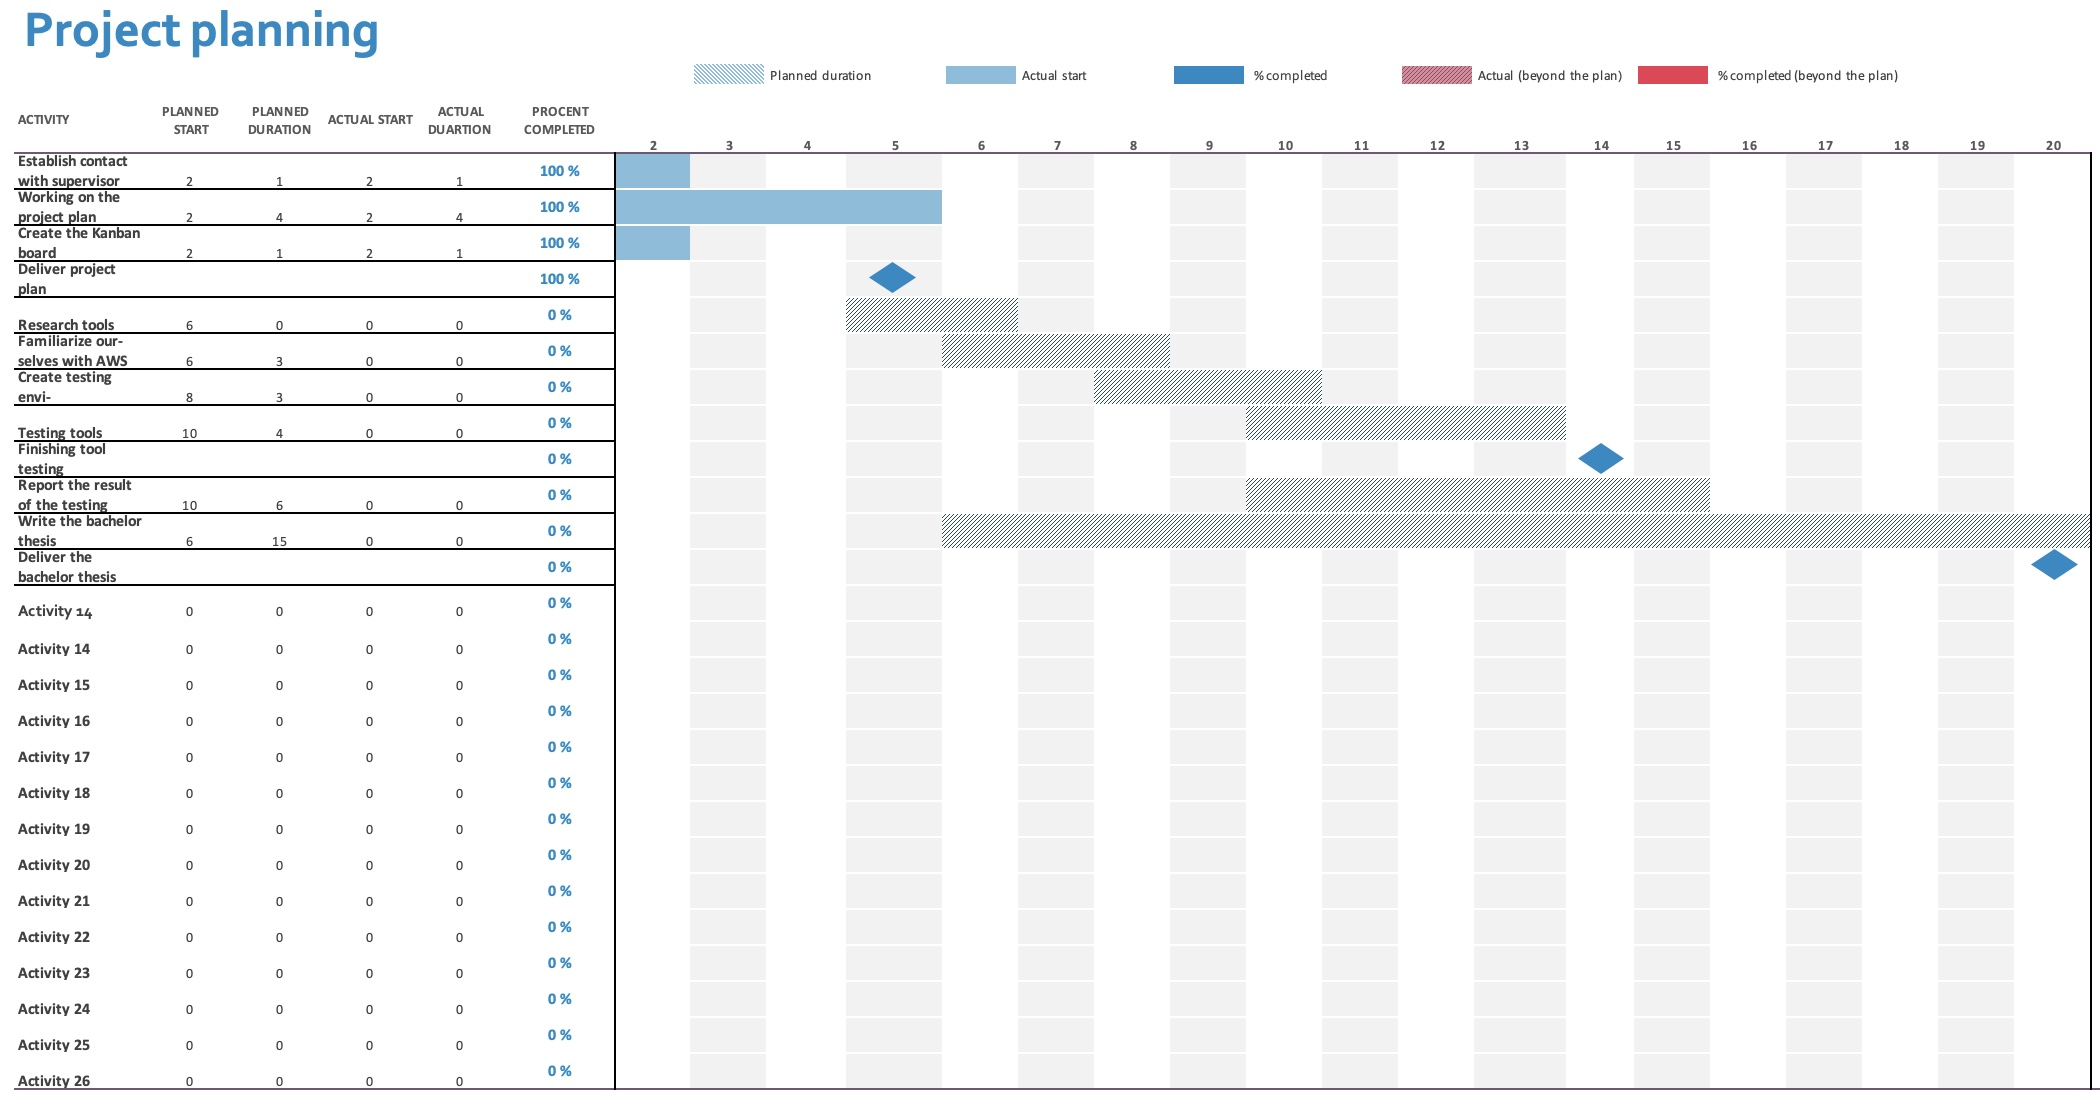
\includegraphics[width=0.8\columnwidth]{Images/gantt2.jpg}
    \caption{Original Gantt Chart}
    \label{fig: Original Gantt Chart}
\end{figure}

% Add a photo of the updated and finished Gantt chart

\subsection{Distribution of Work}
The group decided to divide the work into two parts at the start of the thesis to ensure that the thesis progressed continuously. The first part is practical, and the second is report writing. The responsibilities were assigned based on each group member's strength and what they most desired to do. Every member of the group contributed to the thesis, and everyone worked together to complete the report on time. 


\subsection{Goals}
%diskutere målene vi satt oss (vet ikke om det er nødvendig)



\section{Further Work}

In further work, it could strengthen the thesis to perform a broader analysis of various security tools that perform SAST, DAST, and SCA scans -  where the selected tools are based on these analyses. During these analyses, an assessment can also be made of which requirements must be met in order for a tool to be selected. 

To get an understanding of the whole \acrlong{sdlc}, it would have been relevant to add earlier phases into the thesis to acquire a more complete view of the life cycle and correspond with the shift-left method that prioritizes early testing to detect vulnerabilities sooner. This would demonstrate the shift-left concept, which involves conducting testing as early as feasible in the process.  

\section{Conclusion}
%snakke om hva vi har gjort og hva vi anbefaler 